%----------------------------------------------------
% Setup Beamer
%----------------------------------------------------
\documentclass[hyperref={colorlinks=true}]{beamer}

%----------------------------------------------------
% Packages to use
%----------------------------------------------------
\input{../packages.sty}

%----------------------------------------------------
% Setup Theme
%----------------------------------------------------
\input{../theme.sty}

%----------------------------------------------------
% Table of Contents at each section transition
%----------------------------------------------------

\AtBeginSection[]
{
   \begin{frame}
       \frametitle{Outline}
       \setcounter{tocdepth}{2}
       \tableofcontents[currentsection]
   \end{frame}
}

%----------------------------------------------------
% Colors
%----------------------------------------------------
\input{../mycolors.sty}

%----------------------------------------------------
% Style, formatting, and new commands
%----------------------------------------------------
\newcommand{\CourseYear}   {2024}
\newcommand{\CanvasURL}    {https://canvas.uchicago.edu/courses/58627}
\newcommand{\CanvasLink}   {\href{\CanvasURL}{\CanvasURL}}
\newcommand{\GitHubURL}    {https://github.com/UChicagoPhysics/PHYS250}
\newcommand{\GitHubLink}   {\href{\GitHubURL}{\GitHubURL}}
\newcommand{\PlatformURL}  {https://binderhub.pile.uchicago.edu/}
\newcommand{\PlatformLink} {\href{\PlatformURL}{\PlatformURL}}
\newcommand{\PiazzaURL}    {https://canvas.uchicago.edu/courses/58627/discussion\_topics}
\newcommand{\PiazzaLink}   {\href{\PiazzaURL}{\PiazzaURL}}
\input{../newcommands.sty}
\input{../EandMcommands.sty}

%----------------------------------------------------
% Set paths for plots and images
%----------------------------------------------------
\input{../paths.sty}


%-----------------------------------------------------------------------------------------
% Title: [Column]{Title}
%-----------------------------------------------------------------------------------------
\title[PHYS 250 (Autumn 2024) -- Lecture 3]{The physics of randomness and emergent properties}

%-----------------------------------------------------------------------------------------
% SubTitle: [Column]{Subtitle}
%-----------------------------------------------------------------------------------------
\subtitle{PHYS 250 (Autumn 2024) -- Lecture 3}

%-----------------------------------------------------------------------------------------
% Author: [SubAuthor]{Author}
%-----------------------------------------------------------------------------------------
\author[D.W.~Miller]{David Miller}

%----------------------------------------------------
% Institute: [SubInst]{Institute}
%----------------------------------------------------
\institute[EFI, Chicago] 
{
  Department of Physics and the Enrico Fermi Institute\\
  University of Chicago
}

%----------------------------------------------------
% Institute: [SubInst]{Institute}
%----------------------------------------------------
\date[October 8, 2024]{October 8, 2024}

\subject{PHYS 250 Lecture}

\begin{document}

%==========================================================================================
% TITLE PAGE
%==========================================================================================

{
\begin{frame}
  \titlepage
\end{frame}
}

%==========================================================================================
\section[Final Project]{Final Project}
%==========================================================================================

%-----------------------------------------------------------------------------------------
\subsection[Concept]{Concept}
%-----------------------------------------------------------------------------------------

\begin{frame}%[shrink=10]
  \frametitle{Final Project Concept}

  As mentioned in the first lecture and in the syllabus, there will be a \alertbf{final project for the course} (no exams of any kind).
  
  \vspace{0.3cm}
  
  \begin{ucblock}{Final project  description}
    \begin{itemize}
      \item \bluebf{Individual project}
      \item \bluebf{Focused on a specific physics question with a computational solution, model, calculation, and associated visualization}
      \begin{itemize}
        \item Does \alertbf{not} have to be one of the topics covered in the course
        \item Needs to have a clear physics question and computational approach to its answer
        \item Can be related to work outside of this class. 
        \item I encourage \textit{connections} to other domains as well (statistics, mathematics, engineering, art, music, social science, finance)
      \end{itemize}
      \item \bluebf{Delivered in the form of a \alertbf{poster presentation}}
      \begin{itemize}
        \item \href{http://blogs.lse.ac.uk/impactofsocialsciences/2018/05/11/how-to-design-an-award-winning-conference-poster/}{``How to design an award-winning conference poster''}
        \item \href{https://raw.githubusercontent.com/rafaelbailo/betterposter-latex-template/master/example.png}{``Better'' poster design}
      \end{itemize}
    \end{itemize}
  \end{ucblock}

  
\end{frame}

%-----------------------------------------------------------------------------------------

\begin{frame}%[shrink=10]
  \frametitle{Final Project Ideas and Suggestions}

  A few seeds of an idea for a poster project:

    \begin{itemize}
      \item \bluebf{Randomness and emergent phenomena}
      \begin{itemize}
        \item Develop your own cellular automata simulation (e.g. the Game of Life)
        \item 3D Ising Model
        \item Spin glass model
      \end{itemize}
      \item \bluebf{Numerical Differential equations}
      \begin{itemize}
        \item Solutions of time-dependent Schroedinger equation for two particles
        \item Projectile motion including air resistance / solar wind on satellite motion
      \end{itemize}
      \item \bluebf{Fourier Transforms}
      \begin{itemize}
        \item Sound/image filtering using the FFT and eigenvector pruning
        \item Analysis of similarities between artists, genres, songs using Fourier analysis
      \end{itemize}
      \item \bluebf{Chaotic systems}
      \begin{itemize}
        \item Interactive plots and animations for realistic double pendulum
        \item Dripping faucet
      \end{itemize}
    \end{itemize}

  
\end{frame}

%-----------------------------------------------------------------------------------------
\subsection[Timing]{Timing}
%-----------------------------------------------------------------------------------------

%-----------------------------------------------------------------------------------------

\begin{frame}%[shrink=10]
  \frametitle{Final Project Timeline}

  \begin{columns}
  
  \column{0.6\textwidth}
    
  \begin{ucblock}{Timeline}
    \begin{itemize}
      \item \bluebf{Week 5 -- Tues 29 October:} 1 paragraph project descriptions and sketch of poster due (conceptual design incl. figure ideas)
      \item \bluebf{Week 7 -- Tues 12 November:} Progress report and updated outline of poster due
      \item \bluebf{Week 10 -- Tues 3 December:} Poster due for printing
      \item \bluebf{Week 10 -- Thur 5 December:} Poster session
    \end{itemize}
  \end{ucblock}
  
  \column{0.4\textwidth}
  
  \vspace{-1cm}
  
  \begin{figure}
    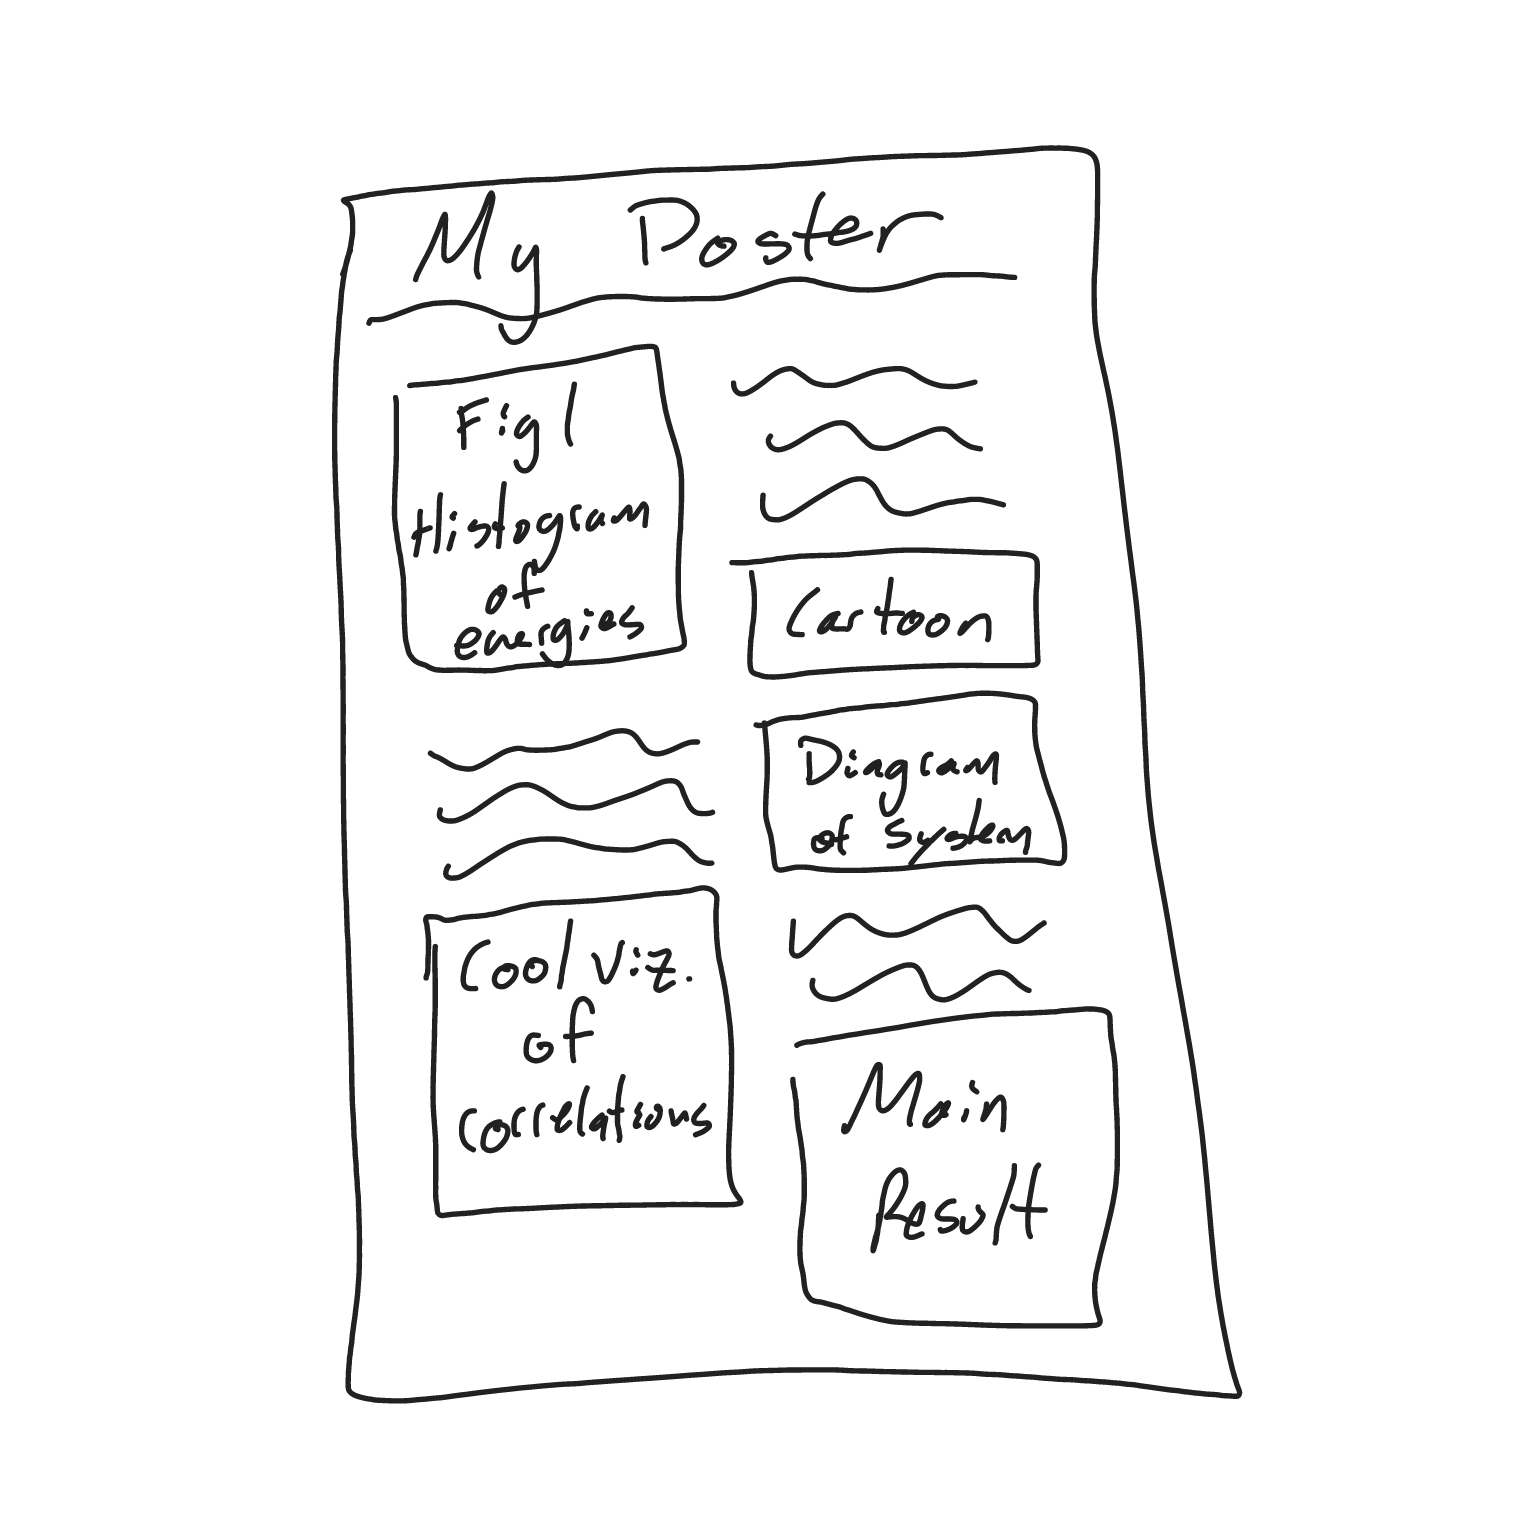
\includegraphics[width=0.9\columnwidth]{PosterConcept.png}\\
    \includegraphics[width=0.6\columnwidth]{/Users/fizisist/Documents/UChicago/Teaching/ComputationalPhysics/PHYS250/PHYS250-Autumn2019/FinalProjects/FinalPosterComputationalPhysics.pdf}\\
  \end{figure}

  
  \end{columns}

  
\end{frame}

%-----------------------------------------------------------------------------------------

\begin{frame}%[shrink=10]
  \frametitle{Poster project example}
  
  \begin{figure}
    \includegraphics[width=0.90\columnwidth]{/Users/fizisist/Documents/UChicago/Teaching/ComputationalPhysics/PHYS250/PHYS250-Autumn2019/FinalProjects/FinalPosterComputationalPhysics.pdf}
  \end{figure}
  
\end{frame}

%==========================================================================================
\section[The physics of randomness and emergent properties]{The physics of randomness and emergent properties}
%==========================================================================================

%-----------------------------------------------------------------------------------------
\subsection[Coin flips]{Coin flips}
%-----------------------------------------------------------------------------------------

\begin{frame}%[shrink=10]
  \frametitle{Coin flips}
  \framesubtitle{See Sethna's text for more info}
  
  We began discussing random numbers last lecture. Let's continue on that topic and extrapolate to much deeper properties of physics.
  
  \vspace{1cm}
  
  Consider flipping a coin and recording the difference $s_N$ between the number of heads and tails found. Each flip contributes $\ell_i = \pm 1$ to the total. 
  
  How big a sum 
  
  \begin{equation} 
    s_N = \sum_{i=1}^{N} \ell_i = \mathrm{(heads - tails)} 
  \end{equation}
  
  do you \alertbf{expect} after $N$ flips? To answer the question regarding \alertbf{expectations}, we need to be able to repeat the measurement many times and compute some statistics about what is going on.
  
\end{frame}


%-----------------------------------------------------------------------------------------

\begin{frame}%[shrink=10]
  \frametitle{Expectation values and statistics}
  
  The average of $s_N$ is not a good measure for the sum, because it is zero (positive and negative steps equally likely). We could measure the average absolute value $\mean{| s_N |}$, but the root-mean-square (RMS) of the sum is better, $\sqrt{\mean{s^2_N}}$. After each flip, the mean square is:
  
  \begin{eqnarray}
    \mean{ s^2_1 } &=& 0.5 (-1)^2 +  0.5 (1)^2 = 1 \\
    \mean{ s^2_2 } &=& 0.25 (-2)^2 +  0.5 (0)^2 + 0.25 (2)^2  = 2 \\
    &\vdots& \\
    \mean{ s^2_N } &=& \mean{ (s_{N-1} + \ell_N)^2 } = \mean{ s^2_{N-1} } + 2 \mean{s_{N-1}\ell_N} + \mean{\ell_N^2}
  \end{eqnarray}
  
  Since $\ell_N = \pm 1$, middle term cancels (equal probability of $\pm1$) and thus
  
  \begin{eqnarray}
    \mean{ s^2_N } &=& \mean{ s^2_{N-1} } + \mean{\ell_N^2} = N - 1 + 1 \\ 
                   &=& N \\
    \sigma_s = \sqrt{\mean{s^2_N}} &=& \sqrt{N}          
  \end{eqnarray}
  
\end{frame}

%-----------------------------------------------------------------------------------------
\subsection[Random walks]{Random walks}
%-----------------------------------------------------------------------------------------

\begin{frame}%[shrink=10]
  \frametitle{Scale invariance and universality}
  
  The discussion above highlights an important point that we will revisit in the case of random ``motion'', or random walks: \bluebf{scale invariance and universality}.
  
  \begin{itemize}
    \item The rate of random $+1$'s and $-1$'s look no different when viewed a ``few'' at a time, or hundreds at a time
    \item On scales where the individual coin tosses are not observable, you cannot pick out any ``preferred'' features
  \end{itemize}
  
  To put this in slightly more concrete terms that will be best studied with random walks
  
  \begin{itemize}
    \item \bluebf{Scale invariance:} the fluctuations of the system occur at all length scales.
    \item \bluebf{Universality:} the behavior of the system is independent of the microscopic details of that system
  \end{itemize}
  
  The latter is also deeply related to the \textbf{central limit theorem}.
  
\end{frame}

%-----------------------------------------------------------------------------------------

\begin{frame}%[shrink=10]
  \frametitle{Random walks}
  
  \begin{columns}

    \column{0.7\textwidth}

    Random walks also arise as trajectories that undergo successive random collisions or turns; for example, the trajectory of a perfume molecule in a sample of air. 
    
    \vspace{0.5cm}    
    
    We will study this example using $N$ fixed length steps:
    
    \begin{itemize}
      \item $\ell_N$: sequence of $N$ steps
      \item $L$: length of each step
      \item $\vec{\ell}_i$: step of length $L$ in the $i$ direction
      \item $d$: number of dimensions
      \item Assume exactly uncorrelated, random steps in each dimension $d$
    \end{itemize}
    
    \column{0.3\textwidth}
    
      \begin{figure}
        \centering
        \includegraphics[width=0.7\columnwidth]{Drunkard.pdf}\\
        \includegraphics[width=\columnwidth]{RandomWalkFractal.pdf}
      \end{figure}
    
  \end{columns}
  
\end{frame}

%-----------------------------------------------------------------------------------------

\begin{frame}%[shrink=10]
  \frametitle{How long of a walk?}
  
  This lack of correlation says that the average dot product between any two steps $\ell_m$ and $\ell_n$ is zero
  
  \begin{equation}
    \mean{\vec{\ell}_m \cdot \vec{\ell}_n} = L \mean{\cos\theta} = 0
  \end{equation}
  
  where $\theta$ is the angle between the two steps. This implies that the dot product of $\vec{\ell}_N$ with $\vec{s}_{N-1} = \sum^{N-1}_{m=1}\vec{\ell}_m$ is zero. Again, we can work by induction:
  
  \begin{eqnarray}
    \mean{ \vec{s}^2_N }  &=& \mean{ (\vec{s}_{N-1} + \vec{\ell}_N)^2 } \\
                          &=& \mean{ \vec{s}\,^2_{N-1} } + \mean{\vec{\ell}_N\,^2} \\ 
                          &=& \mean{ \vec{s}\,^2_{N-1} } + L^2 \\ 
                          &=& N L^2 \\
    \sigma_s = \sqrt{\mean{s^2_N}} &=& \sqrt{N} L         
  \end{eqnarray}
  
  so the RMS distance moved is $\sqrt{N} L$.
  
\end{frame}

%-----------------------------------------------------------------------------------------

\begin{frame}%[shrink=10]
  \frametitle{Markov Chain Monte Carlo}
  
  A random walker is a specific subclass of a more general class of algorithms called \bluebf{Markov chain Monte Carlo (MCMC)}. 
  
  \begin{center}
    \textit{A stochastic model describing a sequence of possible events in which the probability of each event depends only on the state attained in the previous event.}
  \end{center}
  
  \vspace{0.2cm} 
  
  Some characteristics that distinguish this class of algorithms are:   
  
  \begin{itemize}
    \item Sequence of elements chosen from a fixed set using a probabilistic rule
    \item Chain is constructed by adding the elements sequentially
    \item Given the most recently added element, next element only depends on most recent addition
  \end{itemize}
  
  In the case of the random walker, the walker's position after $N$ steps depends on the sequence of steps in the past, and cannot be predicted. However, a pattern emerges for an \alertbf{ensemble} of positions after many such walks.
  
\end{frame}

%-----------------------------------------------------------------------------------------
\subsection[Central limit theorem and analytic descriptions of random behavior]{Central limit theorem and analytic descriptions of random behavior}
%-----------------------------------------------------------------------------------------

\begin{frame}%[shrink=10]
  \frametitle{Central limit theorem}
  
  You're all likely familiar with the central limit theorem:
  
  \begin{center}
    \textit{When independent random variables are added, their properly normalized sum tends toward a normal distribution, even if the original variables themselves are not normally distributed.}
  \end{center}
  
  \begin{figure}
    \centering
    \includegraphics[width=0.45\columnwidth]{Central_limit_theorem.png}
    \includegraphics[width=0.35\columnwidth]{RandomWalk2DEndpoints.pdf}
  \end{figure}
  
  The picture on the right shows the end points of many separate random walks.
  
\end{frame}

%-----------------------------------------------------------------------------------------

\begin{frame}%[shrink=10]
  \frametitle{Diffusion equation}
  
  In cases in which simple behavior seemingly emerges from an ensemble of irregular, jagged random walks (in the continuum limit of long length and time scales) their evolution can be described by the diffusion equation:
  %
  \begin{equation}
    \partialt{\rho} = D \Del^2 \rho = D \partialxsq{\rho}
    \label{eq:diffusion}
  \end{equation}
  
  The diffusion equation can describe the evolving density $\rho(x, t)$ of a local cloud of perfume as the molecules \bluebf{random walk} through collisions with the air molecules. Alternatively, it can describe the probability density of an individual particle as it \bluebf{random walks} through space; if the particles are non-interacting, the probability distribution of one particle describes the density of all particles.
  
\end{frame}

%-----------------------------------------------------------------------------------------

\begin{frame}%[shrink=10]
  \frametitle{Random diffusion (I)}
  
  Consider a general, uncorrelated random walk where at each time step $\Delta t$ the particle's position $x$ changes by a step $\ell$:
  
  \begin{equation}
    x(t + \Delta t) = x(t) + \ell(t).
  \end{equation}
  
  Let the probability distribution for each step be $\chi(\ell)$, which in our case is a discrete probability (e.g. for the 2D random walk, $\chi(\ell) = \delta (|\ell| - L)$ with equal probability in $\pm x, \pm y$). We will assume that $\chi$ has mean zero and standard deviation $a$. The first few moments of $\chi$ are therefore:
  %
  \begin{eqnarray}
    \int \chi(z) dz     &=& 1   \\
    \int z \chi(z) dz   &=& 0   \\
    \int z^2 \chi(z) dz &=& a^2  
  \end{eqnarray}

\end{frame}

%-----------------------------------------------------------------------------------------

\begin{frame}%[shrink=10]
  \frametitle{Random diffusion (II)}
  
  For the particle to go from $x^{\prime}$ at time $t$ to $x$ at time $t+\Delta t$, the step $\ell(t)$ must be $x - x^{\prime}$. This happens with probability $\chi(x - x^{\prime})$ times the probability density $\rho(x^{\prime} , t)$ that it started at $x^{\prime}$. Integrating over original positions $x^{\prime}$, we have:
  %
  \begin{eqnarray}
    \rho(x, t + \Delta t) &=& \int_{-\infty}^{+\infty} \rho(x^{\prime}, t) \chi(x - x^{\prime}) dx^{\prime} \\
                          &=& \int_{-\infty}^{+\infty} \rho(x - z, t) \chi(z) dz
  \end{eqnarray}

  where we have changed variables $x^{\prime} \ra z = x - x^{\prime}$. Now, perform a Taylor expansion in $z$:
  %
  \begin{eqnarray}
    \rho(x, t + \Delta t) &\approx& \rho(x,t) + \frac{1}{2} \partialxsq{\rho} \int z^2 \chi(z) dz \\
                          &\approx& \rho(x,t) + \frac{a^2}{2} \partialxsq{\rho}
  \end{eqnarray}

\end{frame}

%-----------------------------------------------------------------------------------------

\begin{frame}%[shrink=10]
  \frametitle{Slow random diffusion}
  
  If the diffusion is also slow, such that the time derivative of $\rho$ is approximately linear with respect to time and $\rho(x, t + \Delta t) - \rho(x, t) \approx (\partialt{\rho}) \Delta t$, then
  %
  \begin{eqnarray}
    \partialt{\rho} = \frac{a^2}{2 \Delta t} \partialxsq{\rho}.
  \end{eqnarray}

  This is the diffusion equation Eq.~\ref{eq:diffusion} with $D=\frac{a^2}{2 \Delta t}$.
  
  \vspace{0.3cm}
  
  The point is that we obtained an analytical description of a random walk via the diffusion equation under minimal assumptions: the probability distribution is broad and slowly varying compared to the size and time of the individual steps.

\end{frame}


%%==========================================================================================
%\section[Conclusions]{Conclusions}
%==========================================================================================
%
%\begin{frame}%[shrink=1]
%  \frametitle{Conclusions}
%
%  \begin{itemize}
%    \item Something
%  \end{itemize}
%  
%\end{frame}

%==========================================================================================
%==========================================================================================
\end{document}
